\documentclass[11pt,a4paper]{article}

\usepackage[utf8]{inputenc}
\usepackage[T1]{fontenc}
\usepackage{lmodern}
\usepackage{amsmath,amssymb}
\usepackage{geometry}
\usepackage{booktabs}
\usepackage{array}
\usepackage{xcolor}
\usepackage{listings}
\usepackage{graphicx}
\usepackage{hyperref}
\usepackage{parskip}
\usepackage{enumitem}
\usepackage{microtype}

\geometry{margin=2.5cm}
\hypersetup{colorlinks=true, linkcolor=blue!60!black, urlcolor=blue!60!black}
\lstset{basicstyle=\ttfamily\small, columns=fullflexible, keepspaces=true,
        frame=single, rulecolor=\color{black!30}, backgroundcolor=\color{black!3},
        breaklines=true}

\newcommand{\npar}{n_\parallel}
\newcommand{\nperp}{n_\perp}
\newcommand{\code}[1]{\texttt{#1}}

\title{\code{cold\_dispersion}\\[2pt]
  \large Cold-plasma dispersion relation for FP2D\_QLRF\_NL namelists\\
  User manual}
\author{FP2D\_QLRF\_NL tools}
\date{November 2026}

\begin{document}
\maketitle

\section{Purpose}

The quasi-linear RF operator of FP2D\_QLRF\_NL takes the wave as an input:
the perpendicular wavenumber \code{kperp}, the parallel wavenumber \code{kpar}
and the field components \code{eplus}, \code{emin}. \code{cold\_dispersion}
checks those inputs against wave physics. It reads the plasma and RF
parameters of an FP2D namelist, solves the cold-plasma (Stix) dispersion
relation at the namelist $k_\parallel$, and reports for both roots
(fast wave and slow branch):
\begin{itemize}[nosep]
  \item $\nperp^2$ and $k_\perp$ (with wavelength or evanescence length);
  \item the polarisation $E_-/E_+$, $E_y/E_x$, $E_z/E_x$;
  \item a direct comparison with the namelist \code{kperp} and $|\code{emin}/\code{eplus}|$.
\end{itemize}
Optionally it scans the major radius, $B(R)=B_0R_0/R$, and locates the
ion--ion hybrid resonance and the cutoffs.

\section{Files}

\begin{tabular}{@{}>{\ttfamily}l l@{}}
\toprule
cold\_dispersion.f90 & the program (standalone, not part of the \code{.vfproj}) \\
build.bat            & builds \code{cold\_dispersion.exe} with Intel \code{ifx} \\
cold\_example.txt    & example \code{\&COLD} options group \\
plot\_cold\_scan.py  & plots one or more radial scans side by side \\
cold\_dispersion\_manual.tex/.pdf & this manual \\
cold\_scan\_N1\_N2\_fullfield.png & figure of Section~\ref{sec:jet} \\
\bottomrule
\end{tabular}

\section{Build and run}

From a plain \code{cmd} (or PowerShell) prompt:
\begin{lstlisting}
Tools\cold_dispersion\build.bat
\end{lstlisting}
The script calls the Visual Studio 2022 \code{vcvars64.bat} and puts the
oneAPI~2025.2 compiler directories on the paths directly (oneAPI's own
\code{setvars.bat} fails on this machine when \code{vswhere.exe} is not on the
\code{PATH}; the resulting \code{'vswhere.exe' is not recognized} message is harmless).

Running needs the Intel runtime directory on the \code{PATH}:
\begin{lstlisting}
C:\Program Files (x86)\Intel\oneAPI\2025.2\bin
\end{lstlisting}
Then:
\begin{lstlisting}
cold_dispersion.exe  <FP2D namelist>  [<file with an &COLD group>]
\end{lstlisting}
The report goes to standard output. With a radial scan the table is written
in the current directory, as \code{cold\_dispersion-<casename>.txt}.

\section{Input}

\subsection{\code{\&INPUT}: the FP2D namelist}

The program extracts only the variables it needs from the \code{\&INPUT}
group (as text, then an internal namelist read), so any FP2D namelist can be
used unchanged, whatever other entries it holds. Comments (\code{!}) are
allowed.

\begin{tabular}{@{}>{\ttfamily}l p{11cm}@{}}
\toprule
casename & case name, used for the scan file name \\
ne       & electron density (m$^{-3}$) \\
nbulk, xb, ab, zb & bulk ions $k=1\ldots$\code{nbulk}$-1$: density
            \code{ne*xb(k)}, mass number \code{ab(k)}, charge \code{zb(k)} (as in \code{consts.f90}) \\
xpart, aa, za & minority (the FP2D species): density \code{ne*xpart}, mass number, charge \\
b0       & magnetic field (T) at the point of interest \\
frek     & RF frequency (Hz) \\
kpar     & parallel wavenumber (m$^{-1}$), fixes $\npar = c k_\parallel/\omega$ \\
kperp, eplus, emin & used only for the comparison with the computed wave \\
nharm    & harmonic number, used for $\omega/(N\Omega)$ and the plot \\
\bottomrule
\end{tabular}

Masses are $A\,m_p$, as in the FP2D code. Temperatures are not used: the
plasma is cold. Quasi-neutrality $\sum_i Z_i n_i = n_e$ is checked and a
warning printed if it fails.

\subsection{\code{\&COLD}: options (optional)}

The \code{\&COLD} group is read from the second file if one is given,
otherwise from the namelist file itself. It may be appended after the
\code{\&INPUT} group: FP2D reads only \code{\&INPUT}.

\begin{tabular}{@{}>{\ttfamily}l >{\ttfamily}l p{9.5cm}@{}}
\toprule
\textrm{name} & \textrm{default} & meaning \\
\midrule
nu\_omega & 0     & collision frequency$/\omega$, added to every species
                    ($\omega\to\omega+i\nu$); regularises the cold resonances \\
nscan     & 0     & 0: point calculation at $B_0$ only; $>1$: radial scan with this many points \\
r0        & 2.96  & major radius (m) where $B=B_0$ (JET) \\
rmin, rmax & 2.0, 4.0 & scan range (m) \\
nharm\_max & 3    & highest cyclotron harmonic in the layer table \\
\bottomrule
\end{tabular}

The scan assumes a uniform density and $B=B_0R_0/R$; it shows the
structure of the dispersion relation around the heating layer, not a
realistic tokamak profile.

\section{Physics}

\subsection{Dielectric tensor}

Fields vary as $\exp(i\mathbf{k}\cdot\mathbf{r}-i\omega t)$, with
$\mathbf{B}=B\hat z$ and $\mathbf{k}=(k_\perp,0,k_\parallel)$. With
$\Omega_s = Z_s e B/m_s$ (signed, negative for electrons),
$\omega_{ps}^2 = n_s Z_s^2 e^2/(\varepsilon_0 m_s)$ and
$\tilde\omega = \omega + i\nu$:
\begin{align}
R &= 1-\sum_s\frac{\omega_{ps}^2}{\omega(\tilde\omega+\Omega_s)}, &
L &= 1-\sum_s\frac{\omega_{ps}^2}{\omega(\tilde\omega-\Omega_s)}, &
P &= 1-\sum_s\frac{\omega_{ps}^2}{\omega\tilde\omega},
\end{align}
$S=(R+L)/2$, $D=(R-L)/2$. The sum includes electrons, all bulk ions and the
minority; every quantity is also computed \emph{without} the minority
(``bulk only'', Section~\ref{sec:minority}).

\subsection{Dispersion relation}

The wave equation $\mathbf{n}\times(\mathbf{n}\times\mathbf{E})+\mathsf{K}\cdot\mathbf{E}=0$,
with $\mathbf{n}=c\mathbf{k}/\omega$ and $n^2=\nperp^2+\npar^2$, reads
\begin{equation}
\begin{pmatrix}
S-\npar^2 & -iD & \npar\nperp\\
iD & S-n^2 & 0\\
\npar\nperp & 0 & P-\nperp^2
\end{pmatrix}
\begin{pmatrix}E_x\\E_y\\E_z\end{pmatrix}=0 .
\end{equation}
Its determinant gives a quadratic in $x=\nperp^2$ at fixed $\npar$:
\begin{equation}
S\,x^2-\bigl[(S-\npar^2)(S+P)-D^2\bigr]\,x+P\,(R-\npar^2)(L-\npar^2)=0 .
\end{equation}
The two roots are computed in the cancellation-free form
($q=-\tfrac12(b\pm\sqrt{b^2-4ac})$, $x_1=c/q$, $x_2=q/a$), which matters here
because $|P|\sim10^6$ makes the roots differ by three orders of magnitude.
They are sorted by modulus: the smaller is the \textbf{fast wave}, the larger
the \textbf{slow branch} (evanescent in the ICRF for these parameters).
For orientation the program also prints the usual fast-wave estimate
$\nperp^2\approx(R-\npar^2)(L-\npar^2)/(S-\npar^2)$.

$k_\perp=(\omega/c)\sqrt{x}$ is taken on the branch $\mathrm{Re}\,k_\perp\ge0$,
and $\mathrm{Im}\,k_\perp\ge0$ for a purely evanescent root.

\subsection{Polarisation}

Rows 2 and 3 of the wave equation give, for each root,
\begin{equation}
\frac{E_y}{E_x}=\frac{-iD}{S-n^2},\qquad
\frac{E_z}{E_x}=\frac{-\npar\nperp}{P-\nperp^2},\qquad
\frac{E_-}{E_+}=\frac{L-n^2}{R-n^2},
\end{equation}
with $E_\pm=(E_x\pm iE_y)/\sqrt2$. $E_+$ is the left-hand component, rotating
with the ions; these are the \code{eplus} and \code{emin} of the FP2D QL
operator ($E_+$ multiplies $J_{N-1}$, $E_-$ multiplies $J_{N+1}$).

As a check the determinant of the $3\times3$ matrix is evaluated at each root
and printed relative to the size of its terms (\code{check |det|/scale},
$\sim10^{-16}$).

\subsection{The minority and the ``bulk only'' dielectric}\label{sec:minority}

A cold minority makes $L$ singular at $\omega=\Omega_{\rm min}$, so with the
minority included $E_+\to0$ at its fundamental layer, and an ion--ion hybrid
resonance ($S=\npar^2$) and an $L$ cutoff ($L=\npar^2$) appear next to it. In a
hot plasma the singularity is resolved by Doppler broadening and $E_+$ stays
finite. The usual estimate of the polarisation seen by a trace minority is the
one of the majority plasma, so every result is given twice: with all species,
and with the minority left out of the dielectric (``bulk only''). At second
harmonic the minority has no cold resonance and both versions nearly agree.

\section{Output}

\subsection{Report (standard output)}

\begin{enumerate}[nosep]
  \item $B_0$, $f$, $\omega$, $k_\parallel$, $\npar$, $\nu/\omega$;
  \item species table: $Z$, $A$, $n$, $f_p$, $f_c$, $\omega/\Omega_c$, and
        $\omega/(N\Omega_{\rm min})$;
  \item $R, L, S, D, P$ at $B_0$, all species and bulk only;
  \item both roots, all species and bulk only: $\nperp^2$, propagating or
        evanescent, $k_\perp$, $\lambda_\perp$ or decay length,
        $E_-/E_+$, $E_y/E_x$, $E_z/E_x$, determinant check;
  \item comparison with the namelist \code{kperp} and $|\code{emin}/\code{eplus}|$;
  \item positions of the ion cyclotron harmonics, $R = R_0 N\Omega_s(B_0)/\omega$;
  \item with a scan: the sign changes of $S-\npar^2$, $L-\npar^2$, $R-\npar^2$,
        $P$ and of the fast-wave $\mathrm{Re}\,\nperp^2$, each flagged
        \code{zero} (a real layer) or \code{pole} (a cold cyclotron
        singularity, where $|{\cdot}|$ grows towards the crossing).
\end{enumerate}

\subsection{Scan file \code{cold\_dispersion-<casename>.txt}}

Four header lines (\code{\#}), including the namelist \code{kperp},
$|\code{emin}/\code{eplus}|$ and \code{nharm}, then one line per radius:

\begin{tabular}{@{}r l@{}}
\toprule
column & content \\
\midrule
1, 2   & $R$ (m), $B$ (T) \\
3      & $\omega/\Omega_{\rm min}$ \\
4, 5   & Re, Im $\nperp^2$ fast wave (all species) \\
6, 7   & Re, Im $\nperp^2$ slow branch (all species) \\
8, 9   & Re, Im $k_\perp$ fast wave (m$^{-1}$) \\
10     & $|E_-/E_+|$ fast wave \\
11, 12 & Re $\nperp^2$ and $|E_-/E_+|$ of the fast wave, bulk only \\
13--16 & Re$(S-\npar^2)$, Re$(L-\npar^2)$, Re$(R-\npar^2)$, Re $P$ \\
\bottomrule
\end{tabular}

The roots are sorted by modulus at each radius, so near an ion--ion hybrid
resonance the ``fast'' and ``slow'' labels can exchange.

\subsection{Plot}

\begin{lstlisting}
python plot_cold_scan.py scan1.txt [scan2.txt ...] -o out.png
\end{lstlisting}
One column per scan; rows: fast-wave $\mathrm{Re}\,\nperp^2$ (symlog),
$k_\perp$ (propagating only) and $|E_-/E_+|$, all species (blue) and bulk only
(orange). Solid vertical lines mark the minority harmonics, the dashed line
$B=B_0$; dotted horizontal lines the namelist \code{kperp} and
$|\code{emin}/\code{eplus}|$.

\section{Example: the JET minority cases}\label{sec:jet}

Three cases: the namelist \code{jet\_RF\_case1.txt} ($N=1$, $B_0=3.45$\,T, 51\,MHz),
the namelist \code{jet\_RF\_case2\_half\_field.txt} ($N=2$, $B_0=1.725$\,T, 51\,MHz), both
with $n_e=3\times10^{19}$\,m$^{-3}$, 5\% H in D and $k_\parallel=8$\,m$^{-1}$,
plus an $N=2$ full-field variant ($B_0=3.45$\,T, $f=103.6$\,MHz, otherwise the
same), run with
\begin{lstlisting}
&COLD nscan=2001, r0=2.96, rmin=1.9, rmax=4.0 /
\end{lstlisting}

\begin{figure}[h]
  \centering
  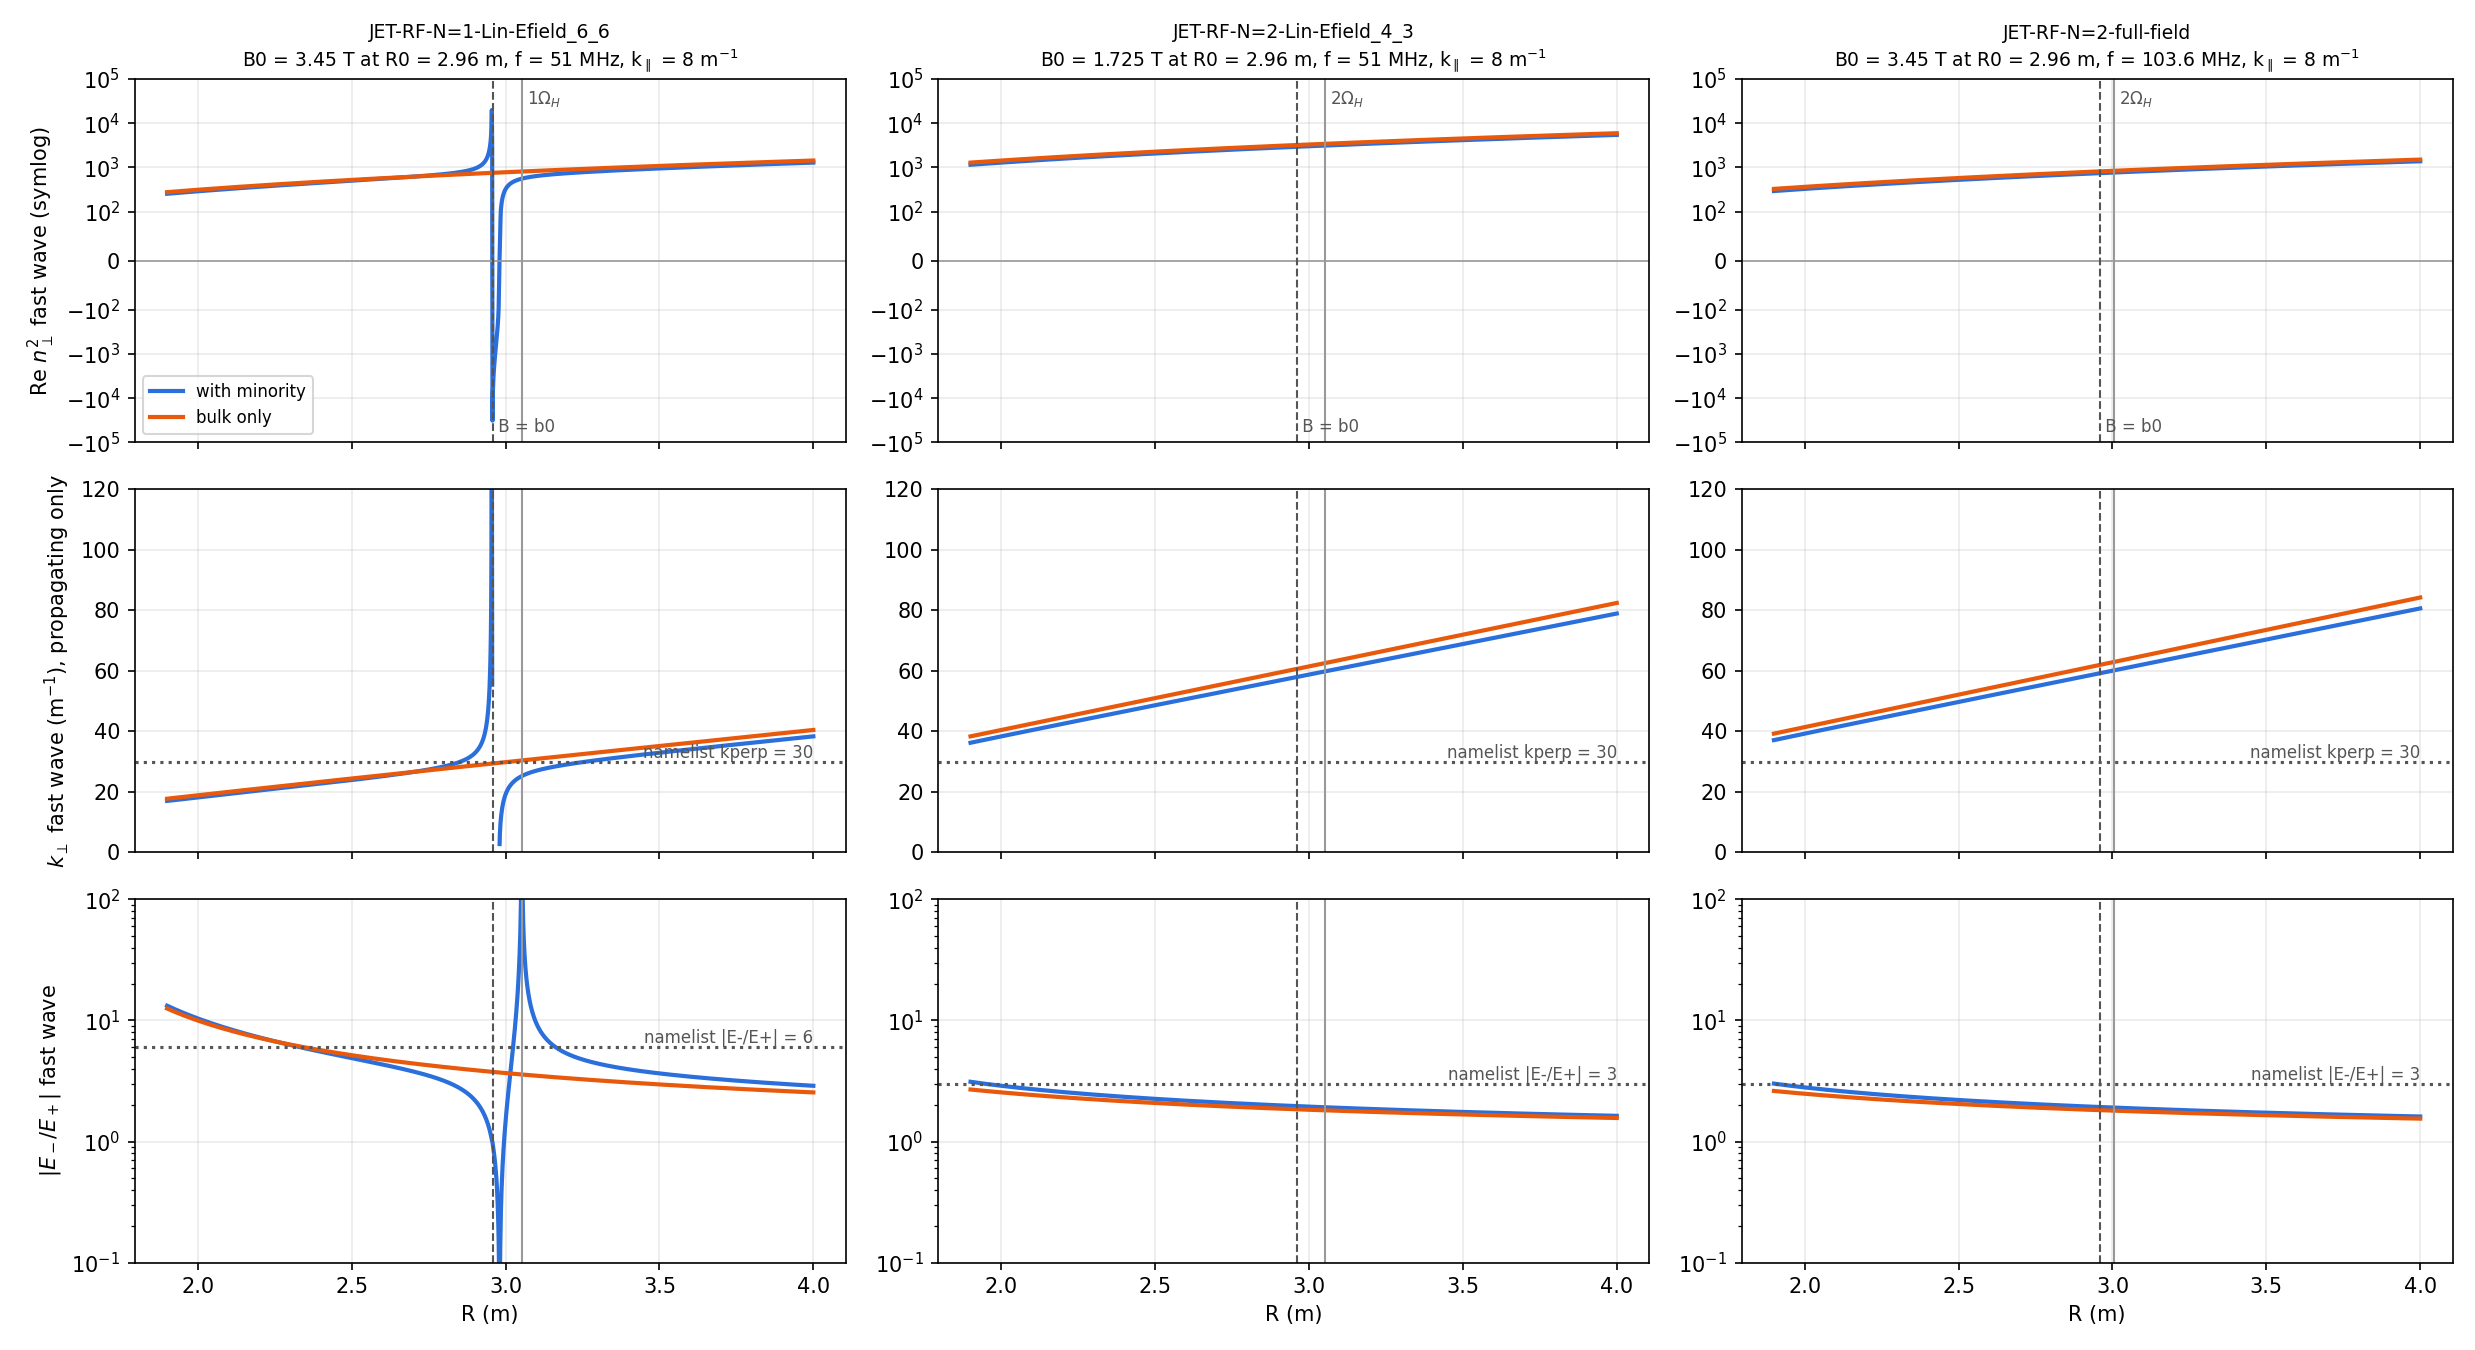
\includegraphics[width=\textwidth]{cold_scan_N1_N2_fullfield.png}
  \caption{Radial scans for the three JET cases. Blue: all species; orange:
  bulk only (minority left out of the dielectric).}
  \label{fig:jet}
\end{figure}

\begin{table}[h]
\centering
\begin{tabular}{@{}l c c c c@{}}
\toprule
 & \multicolumn{2}{c}{$k_\perp$ (m$^{-1}$)} & \multicolumn{2}{c}{$|E_-/E_+|$} \\
\cmidrule(lr){2-3}\cmidrule(l){4-5}
case (all species / bulk only) & fast wave & namelist & fast wave & namelist \\
\midrule
$N=1$, 3.45\,T, 51\,MHz     & -- / 29.4   & 30 & -- / 3.75   & 6 \\
$N=2$, 1.725\,T, 51\,MHz    & 58.0 / 60.6 & 30 & 1.96 / 1.85 & 3 \\
$N=2$, 3.45\,T, 103.6\,MHz  & 59.2 / 62.0 & 30 & 1.93 / 1.82 & 3 \\
\bottomrule
\end{tabular}
\caption{Values at $B=B_0$. For $N=1$ the all-species fast wave is evanescent at $B_0$ (see below).}
\end{table}

Points to note:
\begin{itemize}
  \item $N=1$: the namelist \code{kperp} matches the cold fast wave. With the
        minority included, $B_0$ falls between the ion--ion hybrid resonance
        ($R=2.956$\,m) and the $L$ cutoff ($2.980$\,m), an artefact of the
        cold minority; the bulk-only values are the relevant ones.
        $|E_-/E_+|=6$ is reached only at $R\approx2.3$\,m.
  \item $N=2$: no cold resonance or cutoff near $2\Omega_H$. The fast-wave
        $k_\perp$ is about twice the namelist value and $|E_-/E_+|\approx1.9$.
  \item Full field and double frequency give nearly the same result as half
        field: $\omega/\Omega_i$ is the same for every ion, so the
        dielectric changes little.
\end{itemize}

\section{Verification}

The roots and the polarisation of all three cases were reproduced to every
printed digit by an independent numpy calculation, which builds the full
$3\times3$ wave matrix, fits its determinant as a quadratic in $\nperp^2$, and
takes $\mathbf{E}$ from its null vector (SVD).

\section{Limitations}

\begin{itemize}[nosep]
  \item Cold plasma: no thermal effects, no Doppler broadening, no cyclotron
        or Landau damping, no ion Bernstein waves. Cold singularities at
        $\omega=\Omega_s$ are physical only as markers; use \code{nu\_omega}
        or the bulk-only results there.
  \item Uniform density and $B\propto1/R$ in the scan; no toroidal
        geometry, no density profile.
  \item The ``fast''/``slow'' labels follow $|\nperp^2|$ and may exchange
        across a mode-conversion layer.
\end{itemize}

\end{document}
